%%%%%%%%%%%%%%%%%%%%%%%%%%%%%%%%%%%%%%%%%
% Beamer Presentation
% LaTeX Template
% Version 1.0 (10/11/12)
%
% This template has been downloaded from:
% http://www.LaTeXTemplates.com
%
% License:
% CC BY-NC-SA 3.0 (http://creativecommons.org/licenses/by-nc-sa/3.0/)
%
%%%%%%%%%%%%%%%%%%%%%%%%%%%%%%%%%%%%%%%%%

%----------------------------------------------------------------------------------------
%	PACKAGES AND THEMES
%----------------------------------------------------------------------------------------

% !TeX program = lualatex

\documentclass{beamer}

\newcommand\mybeamerex[2]{%
  \newtheorem*{#1}{#2}%
  \AtBeginEnvironment{#1}{%
     \setbeamercolor{block body}{fg=black,bg=green!5}%
     \setbeamercolor{block title}{fg=white,bg=green!65!black}%
  }%
}

\mode<presentation> {

% The Beamer class comes with a number of default slide themes
% which change the colors and layouts of slides. Below this is a list
% of all the themes, uncomment each in turn to see what they look like.

%\usetheme{default}
%\usetheme{AnnArbor} %no
%\usetheme{Antibes}
%\usetheme{Bergen} %no
%\usetheme{Berkeley} %no
%\usetheme{Berlin}
%\usetheme{Boadilla}
%\usetheme{CambridgeUS}
%\usetheme{Copenhagen}
%\usetheme{Darmstadt}
%\usetheme{Dresden}
%\usetheme{Frankfurt}
%\usetheme{Goettingen}
%\usetheme{Hannover}
%\usetheme{Ilmenau}
%\usetheme{JuanLesPins}
%\usetheme{Luebeck}
%\usetheme{Madrid}
%\usetheme{Malmoe}
%\usetheme{Marburg}
\usetheme{Montpellier}
%\usetheme{PaloAlto}
%\usetheme{Pittsburgh}
%\usetheme{Rochester}
%\usetheme{Singapore}
%\usetheme{Szeged}
%\usetheme{Warsaw}

% As well as themes, the Beamer class has a number of color themes
% for any slide theme. Uncomment each of these in turn to see how it
% changes the colors of your current slide theme.

%\usecolortheme{albatross}
%\usecolortheme{beaver}
%\usecolortheme{beetle}
%\usecolortheme{crane}
\usecolortheme{dolphin}
%\usecolortheme{dove}
%\usecolortheme{fly}
%\usecolortheme{lily}
%\usecolortheme{orchid}
%\usecolortheme{rose}
%\usecolortheme{seagull}
%\usecolortheme{seahorse}
%\usecolortheme{whale}
%\usecolortheme{wolverine}

%\setbeamertemplate{footline} % To remove the footer line in all slides uncomment this line
%\setbeamertemplate{footline}[page number] % To replace the footer line in all slides with a simple slide count uncomment this line

%\setbeamertemplate{navigation symbols}{} % To remove the navigation symbols from the bottom of all slides uncomment this line
}

\usepackage{graphicx} % Allows including images
\usepackage{booktabs} % Allows the use of \toprule, \midrule and \bottomrule in tables
\usepackage{tikz}

\usepackage{wrapfig}

\usepackage{pgfplots}

\definecolor{light-gray}{gray}{0.8}

\usepackage{scalefnt}
\usepackage{etoolbox}
\usepackage{ragged2e}

\apptocmd{\frame}{}{\justifying}{} % Allow optional arguments after frame.


%----------------------------------------------------------------------------------------
%	TITLE PAGE
%----------------------------------------------------------------------------------------

\title{2nd place solution for Actuarial Loss Prediction} % The short title appears at the bottom of every slide, the full title is only on the title page

\author{A. Guly\'{a}s \& N. Fornasin} % Your name
\institute[ALU] % Your institution as it will appear on the bottom of every slide, may be shorthand to save space
{
Team Boosted Goose\\ % Your institution for the title page
\medskip
%\textit{john@smith.com} % Your email address
}
\date{\quad} % Date, can be changed to a custom date

\begin{document}

\begin{frame}
\titlepage % Print the title page as the first slide
\end{frame}

%\begin{frame}
%\frametitle{The $a$ invariant under cone-edge degeneration} % Table of contents slide, comment this block out to remove it
%\tableofcontents % Throughout your presentation, if you choose to use \section{} and \subsection{} commands, these will automatically be printed on this slide as an overview of your presentation
%\end{frame}

%----------------------------------------------------------------------------------------
%	PRESENTATION SLIDES
%----------------------------------------------------------------------------------------

%------------------------------------------------
%\section{Introduction} % Sections can be created in order to organize your presentation into discrete blocks, all sections and subsections are automatically printed in the table of contents as an overview of the talk
%------------------------------------------------


%------------------------------------------------

%------------------------------------------------

\section{Overview}
\begin{frame}
\frametitle{Model overview}
Our model can be divided into three mutually independent blocks:
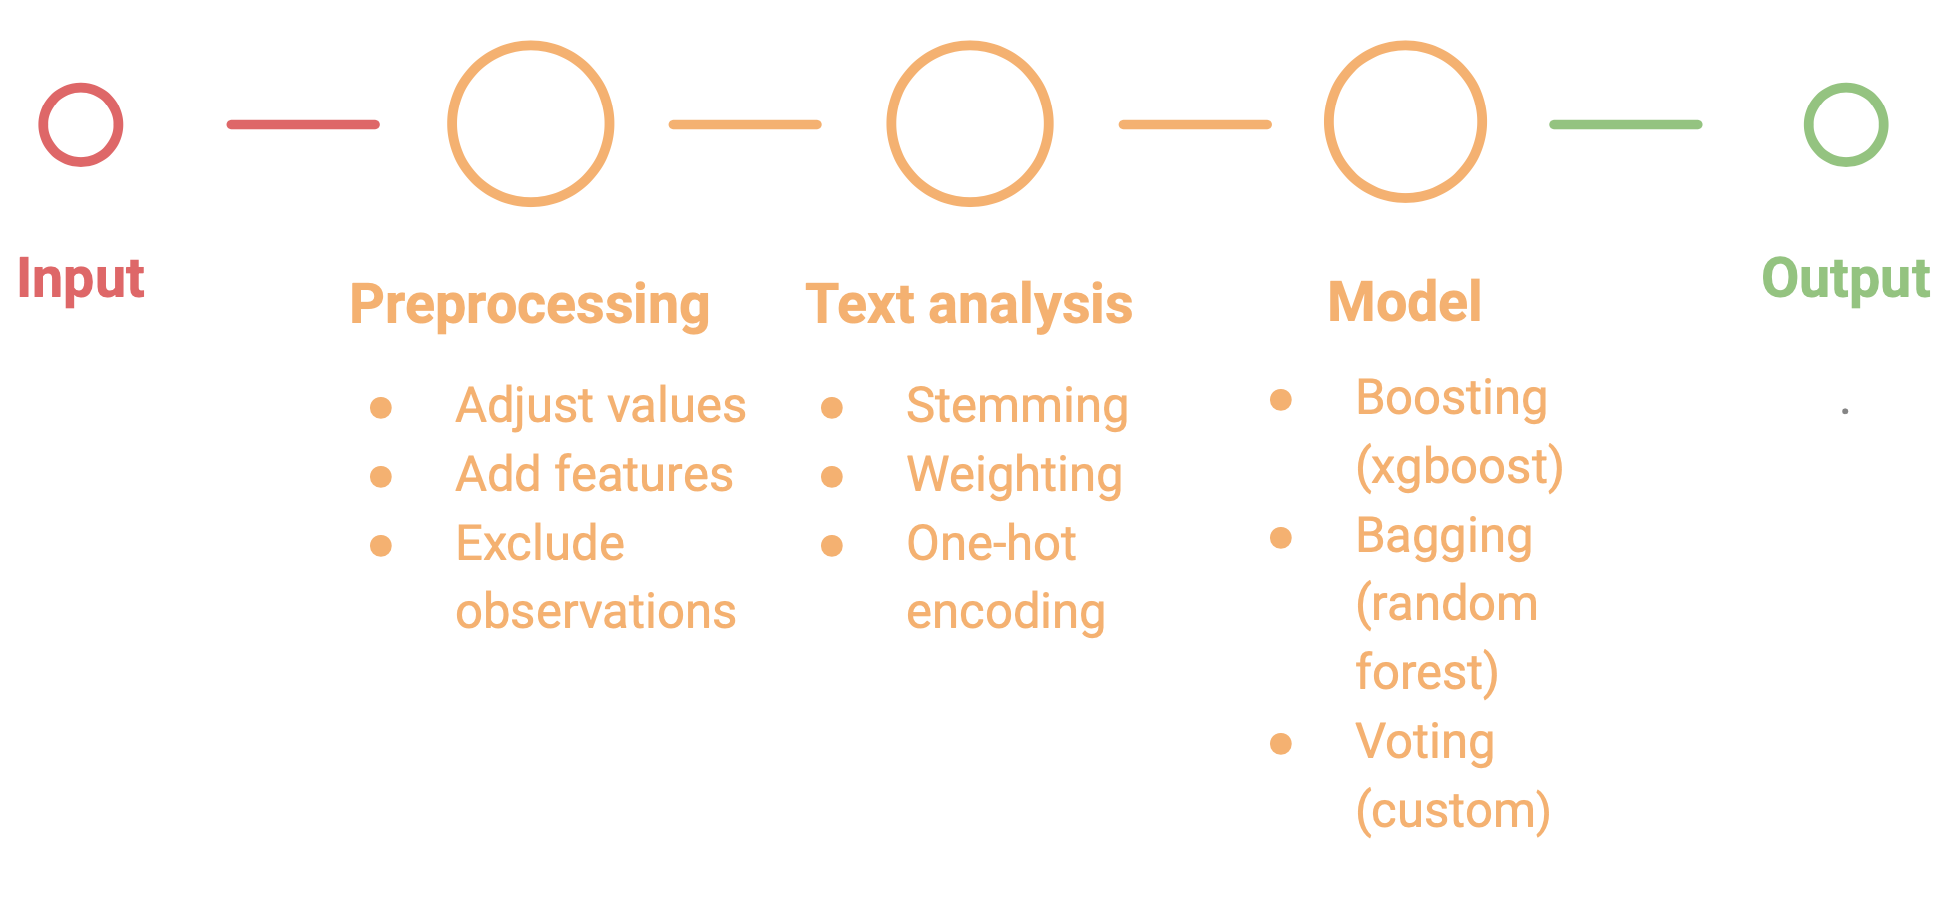
\includegraphics[width=\textwidth]{./images/modeldiagram.png}
\end{frame}

%----------------------------------------------------------------------------------------

\section{Preprocessing}
%\subsection*{The $a$ invariant}
\begin{frame}
\frametitle{Preprocessing}
The preprocessing consisted of the following major steps (purely technical steps are not listed):
\begin{itemize}
\item \textbf{Adjusted unrealistic values} of the predictors, e.g. 200 hours worked per week, reporting date before accident date, etc.
\item \textbf{Added features}, such as: weekday of accident, core working hours, reporting delay, etc.
\item \textbf{Excluded observations} with implausible set of predictors
\end{itemize}
\end{frame}

%------------------------------------------------

\section{Text analysis}
\begin{frame}
\frametitle{Text analysis}
Our analysis of the claim description feature:
\begin{itemize}
\item \textbf{Extraction and stemming} of the most common words (in this step laceration and lacerated both become "lacer")
\item \textbf{Clustering and weighting} of the words according to median ultimate claim cost
\item \textbf{One hot encoding} for every single word identified
\end{itemize}


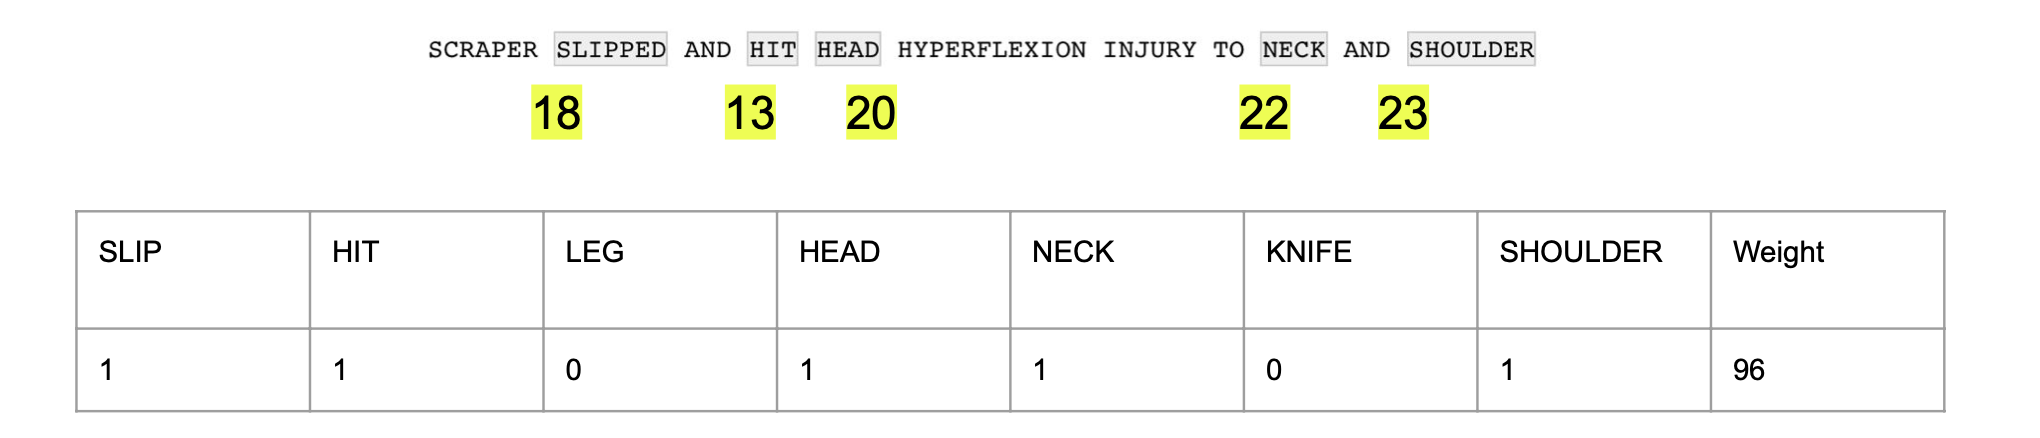
\includegraphics[width=\textwidth]{./images/claimdescription.png}
\end{frame}

%------------------------------------------------

\section{Model}
\begin{frame}
\frametitle{Model}
The algorithm relied on the following ensemble techniques:
\begin{itemize}
	\item \textbf{Boosting}: gradient boosting using xgboost
	\item \textbf{Bagging}: radom forest as base learner
	\item \textbf{Voting}: custom combination based on insight
\end{itemize}
Further details:
\begin{itemize}
	\item Natural logarithm as link function
	\item Tweedie distribution of errors
	\item Monotonic constraints for selected features, e.g. WeeklyWages
\end{itemize}
\end{frame}

\end{document} 